
\section{Review of Heavy Tailed Self-Regularization}
\label{sxn:theory-review}

%n this section, we will briefly review results from Universality that will be relevant for our analylsis.
Let us briefly review our recent Theory of Heavy Tailed Self-Regularization (HT-SR)\cite{MM18_TR}.
\michael{We need to push the other 10 pager to the archive, without the supplementary information}

Write the Energy Landscape (or optimization function) for a typical DNN with $L$ layers, with activation functions $h_{l}(\cdot)$, and with $N\times M$ weight matrices $\mathbf{W}_{l}$ and biases $\mathbf{b}_{l}$, as follows:
\begin{equation}
E_{DNN}=h_{L}(\mathbf{W}_{L}\times h_{L-1}(\mathbf{W}_{L-1}\times h_{L-2}(\cdots)+\mathbf{b}_{L-1})+\mathbf{b}_{L})  .
\label{eqn:dnn_energy}
\end{equation}
%WLOG,
Typically, this model would be trained on some labeled data $\{d_{i},y_{i}\}\in\mathcal{D}$, using Backprop, by minimizing the loss $\mathcal{L}$.
For simplicity, we do not indicate the structural details of the layers (e.g., Dense or not, Convolutions or not, Residual/Skip Connections, etc.). 
Each layer is defined by one or more layer 2D weight matrices $\mathbf{W}_{L}$, and/or the 2D feature maps $\mathbf{W}_{i,L}$ extracted from 2D Convolutional layers.
(We have not yet analyzed LSTM or other complicated Layers.) 
A typical modern DNN may have anywhere between 5 and 5000 2D $\mathbf{W}_{L,i}$ layer matrices.  \footnote{Some notational conventions:
For each Linear Layer, we get a  single, $(N\times M)$ (real valued) 2D matrix, layer weight matrix, denoted $\mathbf{W}_{L}$, for layer $L$.  
This also includes Dense or Fully Connected (FC) layers, as well as 1D Convolutional (Conv1D) layers, Attention matrices, etc.
We ignore the bias here terms $\mathbf{b}_{L}$ in this analysis. 
%XXX.  WHY, WHAT.   
Let the aspect ratio be $Q=\frac{N}{M}$, with $Q\ge 1$.
For the 2-D Convolutional (Conv2D) layers, we have a 4-index Tensor, of the form $(N\times M \times c\times d)$, consisting
of $c\times d$ 2D feature maps of shape $(N\times M)$.    
We  extract $n_{L}=c\times d$ 2D weight matrices $\mathbf{W}_{L,i}$, one for each feature map $i=[1,\dots,n_{L}]$ for layer $L$.}
   
%By Universal behavior, we mean that the eigenvalue spectrum associated weight matrices 
%We can identify different Universality classes 
In the HT-SR Theory, we analyze the eigenvalue spectrum of the associated correlation matrices~\cite{MM18_TR}
in order to character the amount of correlation, and therefore implicit self-regularizartion, present in the DNN.
For each layer weight matrix, $\mathbf{W}_{L}$, construct the associated $M\times M$ (uncentered) correlation matrix $\mathbf{X}$. 
Dropping the $L$ and $l,i$ indices, we have
$$
\mathbf{X} = \frac{1}{N}\mathbf{W}^{T}\mathbf{W}.
$$
%In theoretical treatments, $\gamma$ depends on the form of $\Probab{W_{i,j}}$, e.g., the value of $\mu$, in order to prove the existence of the limiting forms of the ESD.
%For MP theory and the Gaussian Universality class, we can set $\gamma=1$, but for the HT Universality classes, we need to set $\gamma=2/\mu$.
%Of course, empirically, we do not know the PL exponent $\mu$, or the particular Universality class, \emph{a priori}, and the data are of only finite size.
%This will be very important below. 
%For our empirical analysis, we set $\gamma=1$ and deal with these issues in an \emph{a posteriori} manner. 
Compute the eigenvalue spectrum of $\mathbf{X}$, i.e.,
$$ \mathbf{X}\mathbf{v}_{i}=\lambda_{i}\mathbf{v}_{i} .  $$
The ESD of eigenvalues, $\rho(\lambda)$, is just a histogram of the eigenvalues, formally written as
\begin{equation}
\rho(\lambda)=\sum\limits_{i=1}^{M}\delta(\lambda-\lambda_{i})  .
\label{eqn:eigenval_hist}
\end{equation}

%From HT-RMT theory~\cite{XXX-XXX,XXX-XXX,XXX-XXX,XXX-XXX}, the ESD $\rho(\lambda)$ of a HT matrix will have a HT, taking the form
Using out ST-HT Theory, we can now characterize \emph{the correlations} in the weight matrices by examining their ESD $\rho(\lambda)$.
And it turns out, for  typical, well trained DNN weight matrix, the ESD will almost always have a heavy tail  because it is so strongly correlated.  
It will then take the form of a power law, given as

\begin{equation}
\rho(\lambda)\sim\lambda^{-\alpha}  ,
\label{eqn:eigenval_pl}
\end{equation}
which is (at least) valid within a bounded range of eigenvalues $\lambda\in[\lambda_{min},\lambda_{max}]$.  
\michael{Ques: here, $\alpha$ is theoretical, while below $\alpha$ is fit, so clarify.}
%
We can determine $\alpha$ by fitting the   ESD to a PL, using the commonly accepted Maximum Likelihood (MLE) method of Clauset et al.~\cite{CSN09_powerlaw,ABP14}.
%(((
%\charles{Discuss fact the PL tails are Frechet at finite-size so only need to fit the bulk}
%\michael{Ques: clarify.}
%)))
This method works very well for exponents between $\alpha\in(2,4)$, and is adequate, although imprecise, for smaller and larger $\alpha$. 
%\michael{Ques: careful, $\alpha$ (thoeretical or fitted) or $\mu$ here.}
%%MM%% The fitting method is robust in that it is reasonably insensitive to the the choice of normalization $\gamma=1$.

%%MM%%  \charles{Moved paragraphs around a bit here}\michael{To do.}
%%MM%%  
%%MM%%  \michael{can you please add numbers to these equations:  I use them  in the derivation}\michael{To do.}

\nred{removed this: \paragraph{Simple Random Matrix Models.} }

\charlesX{lead into new plot and image here}

%One might imagine that the matrix elements of $\mathbf{W}$ are drawn from some probability distribution, e.g., a Normal $N(0,\sigma)$ distribution
%\begin{equation}
%\Probab{ W_{i,j} } \sim N(0,\sigma)
%\end{equation}
%with mean $0$ and variance $\sigma$.%
%\footnote{At the start of training, DNN weight matrices typically are approximately Normal.  This has been used by some as an analytically-tractable model for trained DNNs, but it is an empirical question whether this is a good model for very non-random matrices that arise at the end of training modern DNNs.  Empirically, it is not~\cite{MM18_TR}.}
%%MM%% \charlesX{Our imagination here lets us derive seemingly \emph{Universal} expressions for how the correlations should behave, even though $\mathbf{W}$  itself is not at all random. }
%These Gaussian models arise in the well known Marchenko-Pastur (MP) RMT~\cite{XXX-XXX}, as well as the Spiked-Covariance model~\cite{johnstone2009}, which is a perturbative variant of MP-RMT. 
%Empirically, it is know that these Gaussian-based models are useful for understanding older, smallish Neural Networks, such as LeNet5~\cite{MM18_TR}.
%More modern DNNs, however, display very different, more exotic,  Universal, behavior.  

\paragraph{Heavy-Tailed Universality.} 

\charles{EXPLAIN UNIVERSALITY, AS WE USE IT, IN THIS SECTION.  NOTE:  we model the ESD of X, the correlations in W, and therefore
how the data has been learned.  Universality of Power Law exponents is special, and different from Universality in RMT.  We use RMT as a guide
This section contains LOTS OF  NEW information, including the 2 images and the discussion around them.  Notice:  the conv2D maps are HVT, not MT.
So we will need an approach that crosses the 2 Universality classes.  Notice:  W is not itself random, but its ESD lookd like the ESD of an HT RMT.}

\charles{TODO: explain why this is special, in the context of statistical physics / Rg theory, and give
references to SOC.  But, more importantly, use the new figure and tie in discussion below}

%Recent work by Martin and Mahoney
in our previous study of Heavy-Tailed Self Regularization (HT-SR)~\cite{MM18_TR}, we examine the eigenvalue density
$\rho(\lambda)$, or Empirical Spectral  Density (ESD), of the linear weight matrices of very large number of modern, pre-trained, DNNs,
such as the AlexNet, the VGGas a\charlesX{explain this plot, ref to notebook and check in.  
This plot is for ImageNet, includes conv2D feature maps, lots of small alpha, but not as good a fit}

Moreover, smaller exponents appear to be correlated with more self-regularization, and, correspondingly, 
better generalization.

\begin{figure}[!htb]
   \centering
   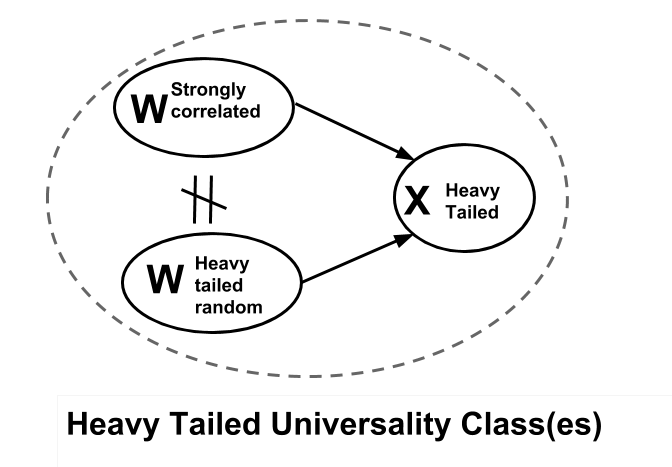
\includegraphics[scale=0.40]{img/universality_classes.png} 
   \caption{}
   \label{fig:universality_diagram}
\end{figure}

\paragraph{Heavy-Tailed Random Matrix Theory.} 

\charles{ THIS SECTION REVIEWS Heavy Tail RMT, and is ALL REVIEW.  
WE MUST  explain how to interpret a correlated ESD in terms of HT-RMT.  BUT be clear that this is not the whole story }

To characterize this behavior, we use a Heavy-Tailed (HT) variant of the MP RMT, where we use
heavy tailed random matrices $\mathbf{W}(\mu)$ to elucidate the different Universality classes.



\begin{equation}
\Probab{ W_{i,j} } \sim \dfrac{W_{0}^{\mu}}{|W_{i,j}|^{1+\mu}}  ,
\label{eqn:ht_dstbn}
\end{equation}
where $W_{0}$ is the typical order of magnitude of $W_{i,j}$, and where $\mu>0$. 
The HT matrix models were first introduced in the SM literature, where they are called \'L\'evy Matrices when $0<\mu<2$~\cite{PB94}.
More generally, there are at least 3 different Universality classes
\footnote{Results for $\mu=2,4$ are slightly different~\cite{SornetteBook,BouchaudPotters03}.  We don't describe them since we don't expect to be able to resolve them numerically.  Also, sometimes L\'evy matrices are split into VHT for $1<\mu<2$ and EHT (Extremely Heavy-Tailed) for $0<\mu<1$, as the properties for these two parameter regimes are somewhat different~\cite{SornetteBook,BouchaudPotters03}.}
of Heavy-Tailed random matrices, defined by the range $\mu$ takes on:
\begin{itemize}
\item $0<\mu<2$: VHT: Universality class of Very Heavy-Tailed (or L\'evy) matrices;
\item $2<\mu<4$: MHT: Universality class of Moderately Heavy-Tailed (or Fat-Tailed) matrices;
\item $4<\mu$: WHT: Universality class of Weakly Heavy-Tailed matrices.
\end{itemize}

\paragraph{Heavy-Tailed, Finite Size Relations} 

\charlesX{THIS SECTION SETS UP IDEAS FOR OUR DERIVATION: 
We have simple relations that apply for both Very Heavy Trailed and Finite Size Fat / Moderately Heavy Tails.  }
\michael{I would derive these 2 relations in the appendix.  To complement our derivation}

For the VHT Universality class, the PL tail of Eqn.~(\ref{eqn:eigenval_pl}) persists in the infinite limit $N\rightarrow\infty$, for $Q$ fixed; and
we have the linear relation between our observed exponent $\alpha$ and the theoretical~$\mu$:
\begin{equation}
\alpha=\frac{1}{2}\mu+1  .
\label{eqn:alpha_mu_vht}
\end{equation}
\michael{Ques: careful, two things change here: observed versus theoretical, and matrix elements versus eigenvalues.}
This expression which works very well at finite size, even for very small matrices $(M,N\approx100)$.
%
For the MHT Universality class, the PL tail of Eqn.~(\ref{eqn:eigenval_pl}) vanishes in the infinite limit $N\rightarrow\infty$, for $Q$ fixed.
\michael{Ques: what does ``vanishes'' mean, it changes slope, and it is MP in the limit for WHT.}
At all finite sizes, however, it persists, and it follows a Frechet distribution (i.e., an exponentially-truncated PL). 
Here, $\alpha$ is still linear in $\mu$, but it displays very strong finite-size effects, giving 
\begin{equation}
\alpha=a\mu+b, 
\label{eqn:alpha_mu_mht}
\end{equation}
where $a,b$ depend strongly on $M,N$. 
(See Table 3 of \cite{MM18_TR} and Figure~\ref{XXX} below for more details on this.)
These strong finite-size effects characterize these MHT distributions; and they are well-known in the SM literature~\cite{SornetteBook,BouchaudPotters03}. 
We will exploit these finite-size effects to develop our-theory.

Finally, for both the VHT and the MHT Universality classes, we expect the maximum empirical eigenvalue, $\lambda_{max}$, to scale with $N$
according to Extreme Value Theory (EVT)~\cite{heavytails2007,Resnick07,MM18_TR}:
\begin{equation}
\lambda_{max}\sim N^{4/\mu-1}  
\label{eqn:scaling_of_lambda_max}
\end{equation}
(where, for simplicity, $Q=1$).
Importantly, \emph{due to HT Universality}, we expect Eqn.~(\ref{eqn:scaling_of_lambda_max}) to hold for matrices in these HT Universality classes (as evidenced by their ESD properties), e.g., DNN weight matrices $\mathbf{W}$ after training, \emph{even when the matrix is not itself a HT random matrix} and therefore not governed by~EVT.



%\section{Using Heavy-Tailed Universality}
\section{Relating Heavy-Tailed Universality to Capacity Metrics}
\label{sxn:theory-new}

In this section, we will describe our main capacity control metric.
%
From prior work~\cite{MM18_TR}, we expect that smaller PL exponents of the ESD imply more regularization and therefore better generalization. 
Since smaller norms of weight matrices often correspond to better capacity control~\cite{LMBx18_TR,SHNx17_TR,PLMx18_TR,BFT17_TR}, we would like to relate the empirical PL exponent $\alpha$ to the empirical Frobenius norm $\Vert\mathbf{W}\Vert_{F}$.
At least na\"{\i}vely, this is a challenge, since smaller PL exponents often correspond to larger matrix norms (and thus worse generalization).
To resolve this apparent discrepancy, we will exploit HT Universality to propose a Universal%
\footnote{To be clear, this metric is Universal, not in the sense that it will apply ``universally'' to every possible DNN, but in the SM sense~\cite{SornetteBook,BouchaudPotters03} that it should apply to matrices broadly, within and across HT ``Universality'' classes.}
DNN Complexity Metric.


\paragraph{Form of a Proposed Universal DNN Complexity Metric.} 

The PL exponent $\alpha$ is a complexity metric for a single DNN weight matrix, with smaller values corresponding to greater regularization~\cite{MM18_TR}.
% The fitted PL  ... AWK
It describes how well that matrix encodes complex correlations in the training data.
Thus, a natural class of complexity or capacity metrics to consider for a DNN is to take a \emph{weighted average} of the PL exponents, $\alpha_{l,i}$, for each layer weight matrix $\mathbf{W}_{l,i}$:
\begin{equation}
\hat{\alpha}:=\dfrac{1}{n}\sum_{l,i}b_{l,i}\alpha_{l,i}  .
\label{eqn:alpha_hat_generic}
\end{equation}
Here, the smaller $\hat{\alpha}$, the better we expect the DNN to represent training data, and (presumably) the better the DNN will generalize to new data.
The question is: what are good weights~$b_{l,i}$?

As we now show, we can extract the weighted average $\hat{\alpha}$ directly from the more familiar Product Norm, by exploiting both Heavy Tailed Universality, and its finite-size effects, arising
in DNN weight matrices.

%%%\paragraph{THEOREM:} \emph{The data dependent VC-like complexity of a Deep Neural Network can be expressed a weighted average the of power law exponents describing the empirical spectral density of the layer weight matrices}
%%
%%%\charles{\paragraph{PROOF:...}}


\paragraph{Product Norm Measures of Complexity.} 

\charlesX{NEED TO CLARIFY 
Worst case Bounds vs Average Case for complexity metrics, and REVIEW MORE OF HIDary's work, either here and/or in the Intro}

It has been suggested that the complexity, $\mathcal{C}$, of a DNN can be characterized by the product of the norms of the layer weight matrices,
$$
\mathcal{C}\sim\Vert\mathbf{W}_{1}\Vert\times\Vert\mathbf{W}_{2}\Vert\cdots\Vert\mathbf{W}_{L}\Vert ,
$$
where $\Vert\mathbf{W}\Vert$ is, e.g., the Frobenius~\cite{XXX-XXX,XXX-XXX,XXX-XXX}.% 
\footnote{Here, we can use either $\Vert\mathbf{W}\Vert$ or $\Vert\mathbf{W}\Vert^{2}$,
%which will make more sense below,
and one can view $\mathcal{C}$ as akin to a data-dependent VC complexity.}
\michael{Cite the most relevant subset of things cited in the intro, including Liao and Srebro.}
%
To that end, we consider a log complexity
\begin{eqnarray*}
\log\mathcal{C} &\sim& \log\bigg[\Vert\mathbf{W}_{1}\Vert\times\Vert\mathbf{W}_{2}\Vert\cdots\Vert\mathbf{W}_{L}\Vert\bigg]  \\
                &\sim& \bigg[\log\Vert\mathbf{W}_{1}\Vert+\log\Vert\mathbf{W}_{2}\Vert\cdots\log\Vert\mathbf{W}_{L}\Vert\bigg]  ,
\end{eqnarray*}
and we define the average log norm of the weight matrices as
\begin{equation}
\langle\log\Vert\mathbf{W}\Vert\rangle=\dfrac{1}{N_{L}}\sum_{L}\log\Vert\mathbf{W}_{L}\Vert  .
\label{eqn:av_log_norm}
\end{equation}
\michael{Ques: is the notation for layers or convolutions or what, be consistent with Eqn.~(\ref{eqn:alpha_hat_generic}).}

\charlesX{Need more references to Hidary's work}

\paragraph{A Universal, Linear,  PL--Norm Relation.} 
Beloew we derive a simple linear relation between the (squared) Frobenius norm $\Vert\mathbf{W}\Vert^{2}_{F}$ of $\mathbf{W}$, the PL exponent $\alpha$, and the maximum eigenvalue $\lambda_{max}$ of $\mathbf{X}$ (i.e., the Spectral Norm $\Vert\mathbf{X}\Vert_{2}=\frac{1}{N}\Vert\mathbf{W}\Vert^{2}_{2}$):  
\begin{equation}
\textbf{PL--Norm Relation:} \quad \alpha\log\;\lambda_{max}\approx\log\;\Vert\mathbf{W}\Vert^{2}_{F}  .
\label{eqn:basic_relation}
\end{equation}
Our justification for using Eqn.~(\ref{eqn:basic_relation}) is three-fold.
\charles{GOOD}
\begin{itemize}
\item First, we can derive Eqn.~(\ref{eqn:basic_relation}) in the special case of very small PL exponent, $\alpha \rightarrow 1$, for (for simplicity) an $N\times M$ random matrix $\mathbf{W}$ (with $N=M$, or $Q=1$).
See Appendix~\ref{sxn:appendix-justify_basic_pl_norm_relation} for this derivation.
\item Second, we observe empirically that multiplying the PL exponent $\alpha$ by $\log\lambda_{max}$ leads to a relation that increases nearly linearly with the (log of the) Frobenius norm for a random HT matrix and that is linearly correlated for real DNN data. 
This is precisely what we want for our simple HT-based complexity metric.
%See Appendix~\ref{sxn:appendix-dnn_versus_random} for these empirical results.
\item Third, based on Universality, we expect this result to extend to larger exponents, both across the VHT Universality class, $\alpha\in(1,2)$, and into the finite-size MHT Universality class, $\alpha\in(2,4)$, where it applies for the finite-size weight matrices in DNNs.
%See Appendix~\ref{sxn:appendix-universality} for more discussion on this point.
\end{itemize}

\charlesX{THE NEXT 2 PARAGRAPHICAL SECTIONS EXPAND ON THE ABOVE POINTS. THE FIRST DISCUSSES THE FACT THAT A RANDOM HT MATRIX HAS A DIVERGING NORM, WHEREAS THE CORRELATED MATRICES HAVE SMALLER NORMS.  THIS IS EXPECTED FROM THEORY ALSO (CITE THE CHICAGO GUYS).  

THE SECOND SECTION PRESENTS THE PL-NORM RELATION, AND SHOWS HOW THE FINITE SIZE EFFECTS ARISE.  TO DO THIS, WE NEED TO PLOT ALPHA LOG LAMBA MAX VS LOG FROBENIUS NOM, SHOW IT IS LINEAR, AND THEN.  DRILL INTO THE SMUDGE .  THIS SECTION SHOULD BEIN THE SPIRIT AS THE SECTION ON THE OTHER 2 RELATIONS THAT WE DEFINE ABOVE IN THE REVIEW, AND THAT WE USE IN THE DERIVATION,. }

\paragraph{Random Pareto versus Strongly Correlated DNN Matrices.} 

We would like a method that applies both to HT Pareto matrices as well as to non-random, indeed strongly-correlated, finite-sized empirical DNN layer weight matrices that (as evidenced by their ESD properties) are in a HT Universality class.  
To accomplish this, however, requires some care: while the pre-trained $\mathbf{W}$ matrices do have ESDs that display empirical signatures of HT Universality~\cite{MM18_TR}, they are \emph{not} random Pareto matrices, and their empirical Frobenius norms behaves very differently than that of a random Pareto matrix.  

To illustrate this,, we generate a large number of  Heavy-Tailed  random matrices $\mathbf{W}^{rand}(\mu,M)$, with different number of eigenvalues $M$ (with aspect ratio $Q=1$), and drawn from a Pareto distribution,
$$
\Pr[{W}^{rand}_{i,j}]\sim\dfrac{1}{x^{1+\mu}}  ,
$$
with exponents $\mu\in[0.5, 5]$.
%
We then fit the ESD of each $\mathbf{W}^{rand}(\mu)$ to a PL using the method of Clauset et al.~\cite{CSN09_powerlaw,ABP14} to obtain the empirical exponent $\alpha$.   Figure~\ref{fig:fnorm} displays the relationship between the (squared) Frobenius norm and the PL exponents, for both randomly-generated Pareto matrices, and the weight matrices
(extracted from the Conv2D Feature Maps) from the pre-trained VGG11 DNN.

\charlesX{paragraph needs point sentence}
For a random Pareto matrix $\mathbf{W}^{rand}(\mu)$, the Frobenius norm $\Vert\mathbf{W}^{rand}(\mu)\Vert_{F}$ increases with decreasing exponent $(\mu)$; there is a modest finite-size effect; and, as the tails of the ESD $\rho(\lambda)$ get heavier, the largest eigenvalue $\lambda_{max}$ of $\mathbf{X}$ scales with the largest element of $\mathbf{W}^{rand}(\mu)$. 
\michael{$\alpha$ or $\mu$ here.}
\michael{Cite something or show this.}
For the weight matrices of a pre-trained DNN, however, the Frobenius norm $\Vert\mathbf{W}\Vert_{F}$ increases with \emph{increasing} exponent $(\alpha)$, saturating at $\alpha\approx 3$.
This happens because, due to the training process, the $\mathbf{W}$ matrices themselves are highly-correlated, and not random matrices with a single large, atypical element;   
and, yet, the ESD $\rho(\lambda)$ of these pre-trained correlations matrices $\mathbf{X}$ display Universal HT behavior~\cite{MM18_TR}.
This is one of the amazing properties of Universality.
XXX.  FIX.

 
 
 \begin{figure}[t] %[!htb]
    \centering
    \subfigure[Random Pareto Matrices] {
        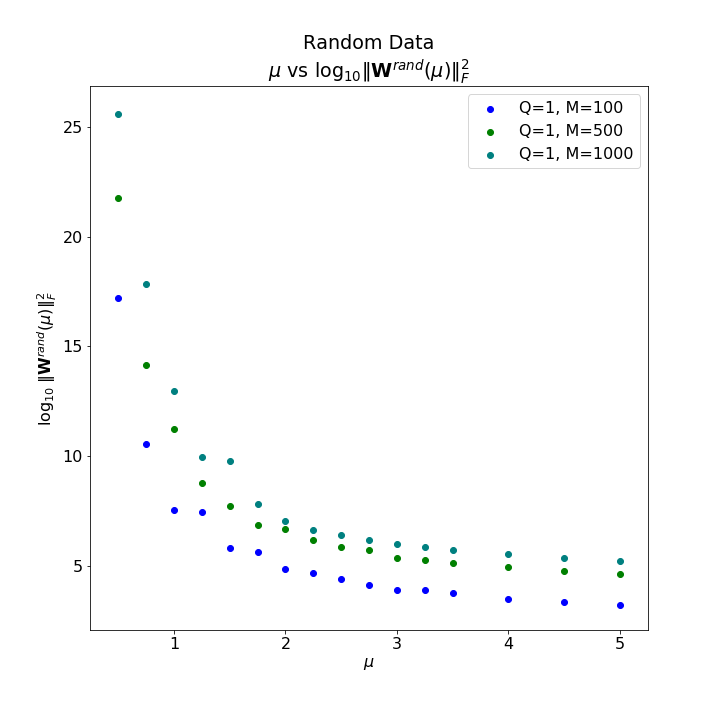
\includegraphics[scale=0.30]{img/fro-rand.png} 
        \label{fig:fro-rand}
    }
    \subfigure[Pre-trained VGG11 Weight Matrices]{
        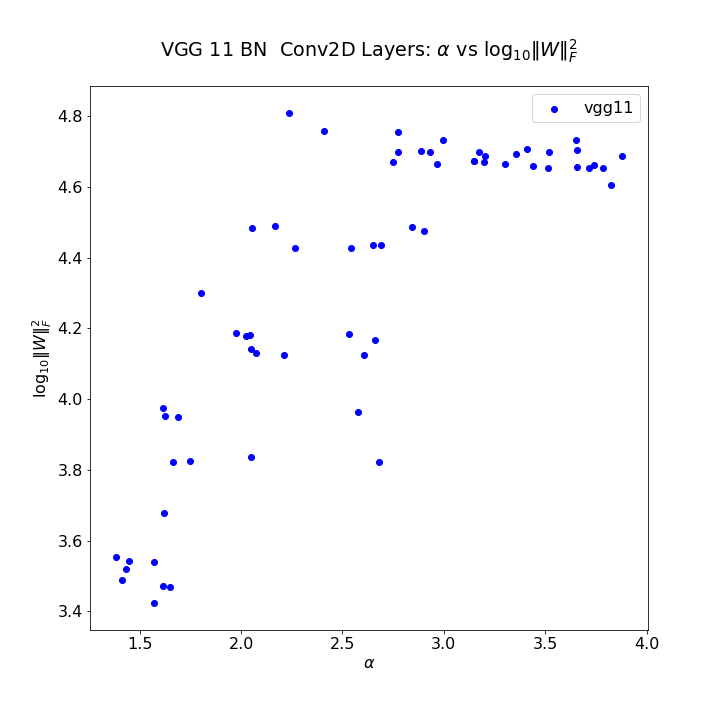
\includegraphics[scale=0.30]{img/fro-vgg11.png} 
        \label{fig:fro-vgg11}
    }
        \caption{Dependence of Frobenius Norm on Power Law exponents for random Pareto versus pre-trained DNN matrices.
                 \michael{Is thie $\alpha$ or $\mu$ for Pareto.} 
                 \michael{Have consistent title naming, here and below.} 
                }
    \label{fig:fnorm}
\end{figure}


\paragraph{NOT SURE WHAT TO CALL THIS SECTION}
\charlesX{LEAD INTO HOW WE GOT THIS EXPRESSION...}

Multiplying $\alpha$ by $\log_{10}\lambda_{max}$, we now have a relation that increases nearly linearly with the 
Frobenius norm for a random matrix, and is linearly correlated for real DNN data. Which is exactly what we want for our simple complexity metric.

'Figure~\ref{fig:randW} displays the Forbenius norm (squared)  as a function of the power law exponent $\alpha$ \nred{(that was fit)}
$$
\dfrac{\log\Vert\mathbf{W}\Vert^{2}_{F}}{\log\lambda_{max}}\;\;vs.\;\;(\alpha)  .
$$

%\paragraph{Numerical Properties of Eqn.~(\ref{eqn:basic_relation}).}

We demonstrate that this relation holds numerically for both Heavy Tailed random matrices and for the weight matrices in pre-trained DNNs, \nred{as above}.
%To understand this relation better, and to sketch a proof,
%we will generate the data for a number of a Heavy-Tailed random matrices, 
%with different power law exponents $\mu$.
%Note that this linear relation holds over several log scales.  However,
%the relation does deviate from linearity at the smaller values of $\alpha\;\log_{10}\;\lambda_{max}$.
%This is readily explained below .  

 \begin{figure}[t] %[!htb]
    \centering
    \subfigure[Random Pareto Matrices] {
        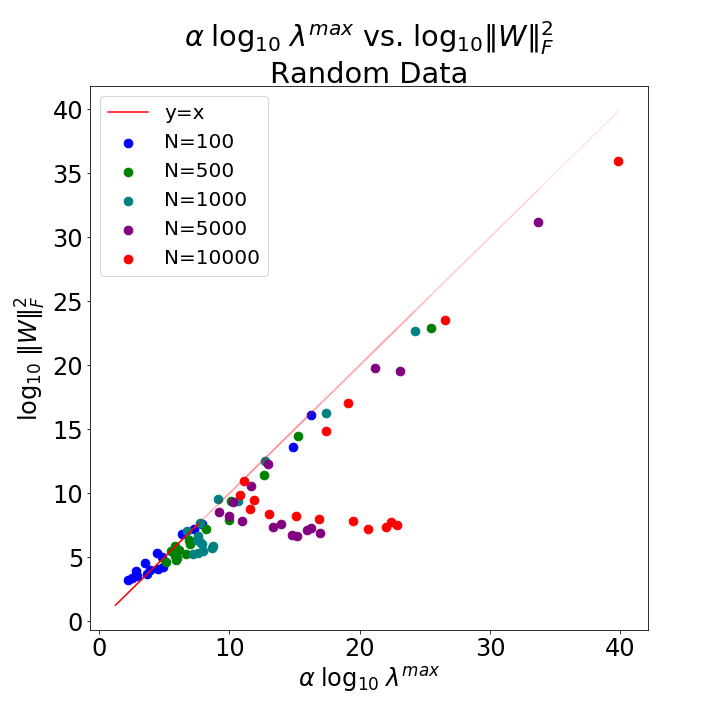
\includegraphics[scale=0.30]{img/relation-rand.png} 
        \label{fig:relation-rand}
    }
    \subfigure[VGG 11 Weight matrices]{
        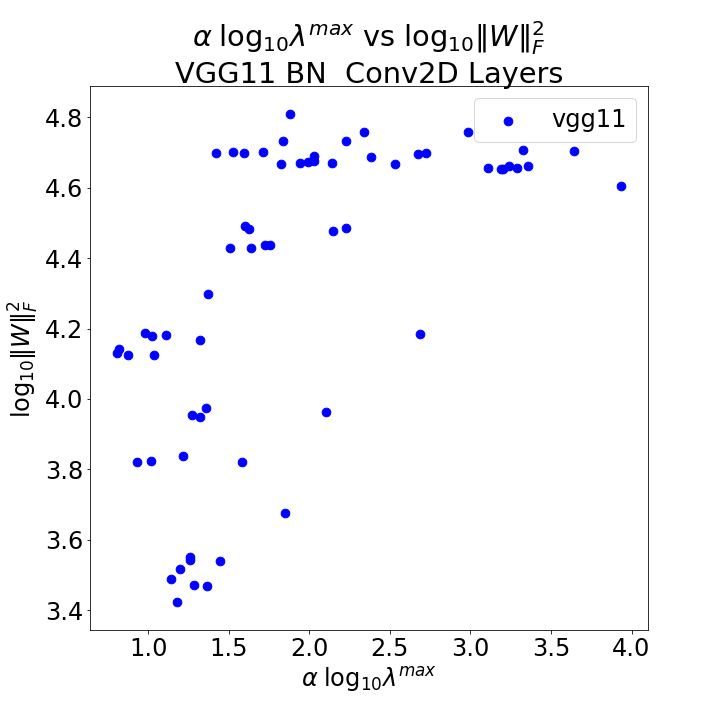
\includegraphics[scale=0.30]{img/relation-vgg11.png} 
        \label{fig:relation-vgg11}
    }
        \caption{Relation between $\alpha\;\log_{10}\;\lambda_{max}$ and the Frobenius Norm squared }
    \label{fig:relations}
\end{figure}

The numerical results for the the Power Law-Norm relation shows several interesting features: 
First, as $\alpha$ increases, we see the relation for
\begin{itemize}
\item  $\alpha<2$ , a near linear relation 
\item  $\alpha>2$ for $N,M$ large, the relation saturates, becoming constant
\item  $\alpha>2$  for smaller $N,M$,  a nearly linear relation, but with strong finite-size effects
\end{itemize}

\charlesX{REPEATED:
These observations lead to a novel linear relation between the Frobenius norm and the power law exponent for our Heavy tailed matrices:
$$
\log\Vert\mathbf{W}\Vert^{2}_{F}\approx\alpha\log\lambda_{max}  ,
$$
which works very well for VHT Levy matrices, $\alpha<2$, and is a good approximation for MHT matrices and even some WHT matrices. 
And we believe this is the first time this relation has been noted in the literature.}


\begin{figure}[t] %[!htb]
   \centering
   \subfigure[$\dfrac{1}{N}$ normalization] {
      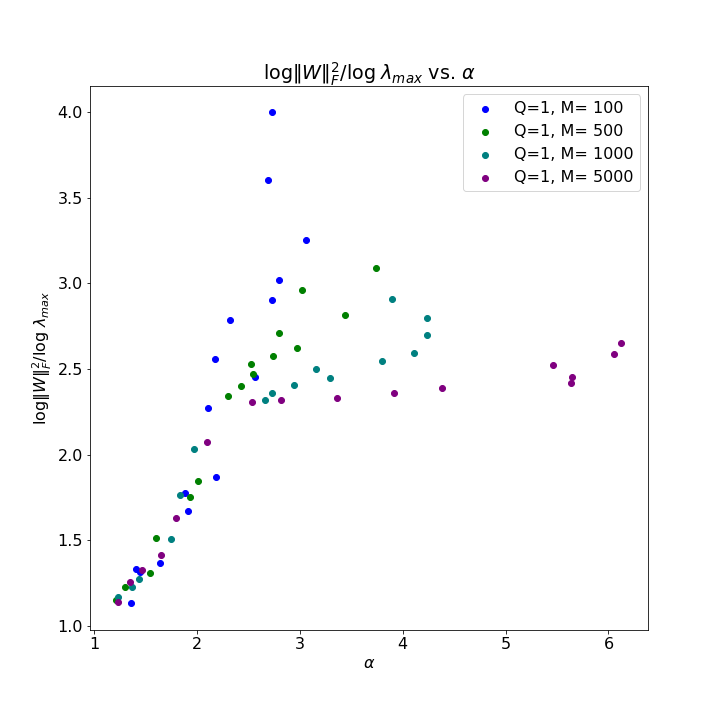
\includegraphics[scale=0.30]{img/Alpha-LogNorm-Relations.png}
      \label{fig:randW}
   }
   \subfigure[$\dfrac{1}{N^{2/\mu}}$ normalization] {
      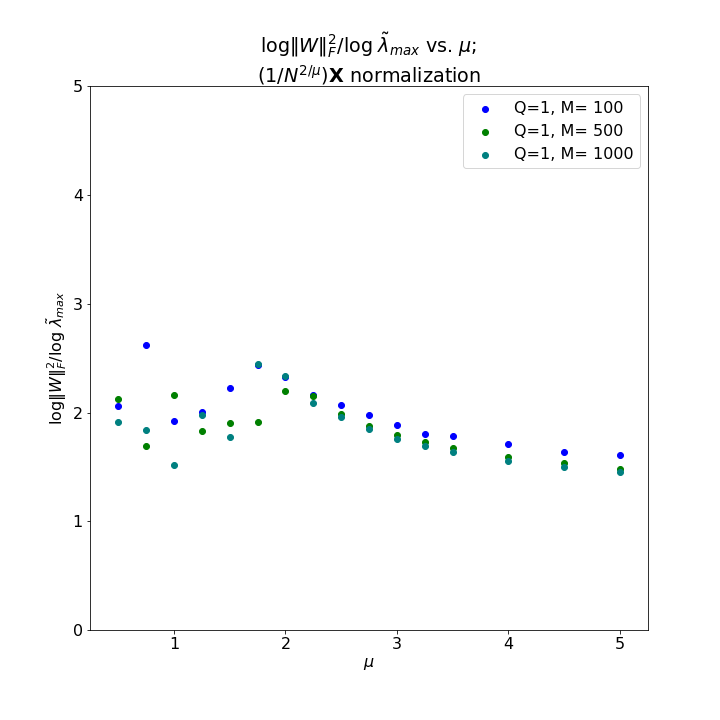
\includegraphics[scale=0.30]{img/LogNorm-Lmax-Scaled.png}
      \label{fig:logNormHat}
   }
   \caption{
            Numerical test of Eqn.~(\ref{eqn:basic_relation}) for random HT matrices; and the effect of different normalizations.
            \michael{Careful about $\alpha$ versus $\mu$ here.}
            \michael{Mention finite-size issues versus saturation.}
           }
\end{figure}


\charlesX{back to old stuyff}

%%MM%% This approximate relation formally only hold in the asymptotic limit of very small power law exponents $\alpha\rightarrow 1$ for
%%MM%% random heavy tailed matrices, but using Universality, we can safely extend it up to the finite-size MHT class, with
%%MM%% exponents $\alpha=4$ (and larger).  

Based on Eqn.~(\ref{eqn:basic_relation}), we will below choose the weights in Eqn.~(\ref{eqn:alpha_hat_generic}) to be the corresponding maximum eigenvalues of $\mathbf{X}$.
Note, however, that Eqn.~(\ref{eqn:basic_relation}) provides an alternate interpretation of the fitted PL exponent.
It is (up to the $\frac{1}{N}$ scaling) approximatelly the Stable Rank in Log-Units:
$$
\mbox{Log-Units Stable Rank:} 
\quad
\mathcal{R}^{log}_{s}:=\dfrac{\log\Vert\mathbf{W}\Vert^{2}_{F}}{\log\lambda_{max}}  \approx \alpha  .
$$


\nred{awkward: \paragraph{A Proposed Universal DNN Complexity Metric.} }

Given Eqn.~(\ref{eqn:basic_relation}), we define the complexity metrics for Linear and Convolutional Layers as follows.
For Linear~Layers:
$$
\text{Linear Layer:}\;\;\log\Vert\mathbf{W}_{L}\Vert^{2}_{F}\rightarrow\log\lambda^{max}_{L}\alpha_{L}  .
$$
\michael{Need to be consistent with superscripts and subscripts, on $\lambda$, in this par and elsewhere.}
For Conv2D Layers, we relate the ``norm'' of the 4-index Tensor $\mathbf{W}_{l}$ to the sum of the $n_{L}=c\times d$ terms for each feature map, giving: 
$$
\text{Conv2D Layer:}\;\;\log\Vert\mathbf{W}_{L}\Vert^{2}_{F}\rightarrow \sum_{i=1}^{n_{L}}\log\lambda^{max}_{i,L}\alpha_{L,i}  .
$$
So, in the expression for the Product Norm for $\log\mathcal{C}$, we can replace each $\log\Vert\mathbf{W}_{L}\Vert$ term for layer $L$ with these above expressions, and take the average over all $N_{\alpha}$  matrices.  This lets us relate the Product Norm complexity metric to the weighted average of PL exponents, giving
$$
2\log\mathcal{C}=\langle\log\Vert\mathbf{W}\Vert^{2}_{F}\rangle\rightarrow\hat{\alpha}  ,
$$ 
where
\begin{equation}
\hat{\alpha}:=\dfrac{1}{N_{\alpha}}\sum_{i,l}\log\lambda^{max}_{i,j}\alpha_{i,l}  .
\label{eqn:alpha_hat_specific}
\end{equation}
\michael{Ques: have we defined $N_{\alpha}$ anywhere, we use subscripts differently elsewhere.}
This expression resembles the more familiar Product Norm, but it accounts for finite-size effects that the Product Norm relation over-estimates.
\michael{Ques: is that true.} \charlesX{probably not}

We can now use $\hat{\alpha}$ to analyze numerous pre-trained DNNs.
We will see that our approach improves on the loose bound provided by the Product Norm, giving a more accurate expression for predicting trends in the average case test accuracy for real-world production-quality DNNs.


